% Langmuir isotherm for molecular adsorption, theta = K p / (1 + K p).
\documentclass[border=4pt]{standalone}
% Shared style for the ch. 10 schematic plots (figures/src/*.tex).
% Build one figure:  lualatex <name>.tex   then see README.md for the PNG step.
\usepackage{amsmath}
\usepackage{pgfplots}
\pgfplotsset{compat=1.18}
\usetikzlibrary{arrows.meta}

\definecolor{matblue}{HTML}{0072BD}
\definecolor{matorange}{HTML}{D95319}

\pgfplotsset{
  schematic/.style={
    width=8cm, height=6.2cm,
    axis lines=left,
    axis line style={-{Stealth[length=2.5mm]}, line width=0.8pt},
    xtick=\empty, ytick=\empty,
    xmin=0, ymin=0,
    clip=false,
    every axis x label/.style={at={(current axis.right of origin)}, anchor=north east, yshift=-4pt},
    every axis y label/.style={at={(current axis.above origin)}, anchor=north east, xshift=-4pt},
    label style={font=\normalsize},
    samples=200,
  },
  curve/.style={line width=1.4pt, color=matblue},
  guide/.style={line width=0.8pt, dashed, color=black!60},
}

\begin{document}
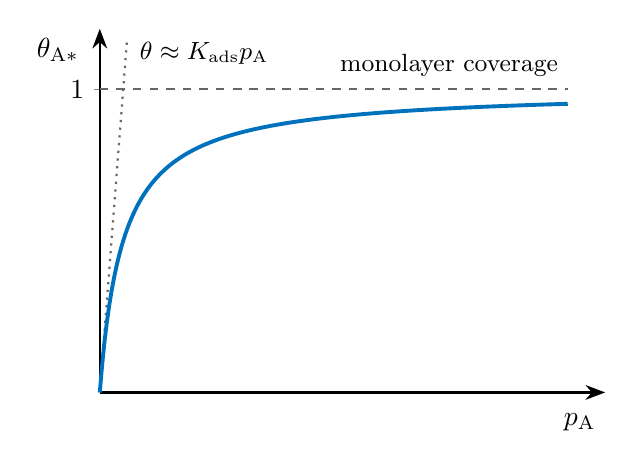
\begin{tikzpicture}
\begin{axis}[schematic, xmax=1.08, ymax=1.2,
    xlabel={$p_\mathrm{A}$}, ylabel={$\theta_{\mathrm{A}\ast}$},
    ytick={1}, yticklabels={$1$}]
  \addplot[guide, domain=0:1] {1};
  \node[anchor=south east, font=\small] at (axis cs:1,1.01) {monolayer coverage};
  \addplot[guide, dotted, domain=0:0.058] {20*x};
  \node[anchor=west, font=\small] at (axis cs:0.065,1.12) {$\theta \approx K_\mathrm{ads}p_\mathrm{A}$};
  \addplot[curve, domain=0:1] {20*x/(1+20*x)};
\end{axis}
\end{tikzpicture}
\end{document}
